\documentclass{article}

% Recommended, but optional, packages for ICLR.
\usepackage{times}
\usepackage[utf8]{inputenc}
\usepackage[T1]{fontenc}
\usepackage{graphicx}
\usepackage{hyperref}
\usepackage{url}
\usepackage{booktabs}
\usepackage{amsmath,amssymb}
\usepackage{iclr2021_conference}
\usepackage{float}
\usepackage{placeins}
\usepackage{tikz}
\usetikzlibrary{positioning}

% Optional math commands
\input{math_commands.tex}
\graphicspath{{../figures/}}

\title{Détection de risques dans les marchés publics (DECP) par analyse de graphes}

\author{\textbf{Nom1} \\ École Centrale Casablanca \\ 
\And
\textbf{Nom2} \\ École Centrale Casablanca \\ 
\And
\textbf{Nom3} \\ École Centrale Casablanca \\ }

\iclrfinalcopy

\begin{document}
\maketitle

\begin{abstract}
Nous étudions les marchés publics français (DECP) sous l’angle des graphes afin d’identifier des relations acheteur–entreprise présentant un risque de comportement collusif. Notre étude se concentre sur les marchés de travaux de construction (CPV 4521) au second semestre 2024. Nous modélisons le système comme un graphe biparti reliant acheteurs et titulaires, où chaque arête représente un marché et porte des attributs (montant, date, nombre d’offres, etc.). À partir de ce graphe, nous construisons des indicateurs simples et interprétables : degrés des nœuds, concentration des montants sur une relation acheteur–titulaire, répétition des interactions et niveau de concurrence (offres reçues). Nous combinons ces signaux dans un score de risque de base, normalisé et pondéré, destiné au tri et à la priorisation des contrôles. Sur 8\,957 marchés filtrés, nous obtenons 5\,491 relations acheteur–titulaire agrégées. Le score de risque présente une distribution à queue, avec un petit ensemble d’arêtes très concentrées et faiblement concurrentielles. Les relations classées “haut risque” (≥ 95e percentile) affichent en moyenne moins d’offres reçues et une forte concentration bilatérale. Nous ne prétendons pas prouver une fraude\,: le score est un outil descriptif d’aide à l’inspection. Nos résultats montrent la pertinence d’une approche par graphes pour la priorisation des contrôles, tout en soulignant la nécessité de données plus riches (soumissionnaires, prix des offres) pour distinguer précisément les types d’entente.
\end{abstract}

\section{Introduction et motivation}
La commande publique représente un enjeu économique et sociétal majeur. Des pratiques d’entente ou de collusion peuvent augmenter les prix, réduire la concurrence et dégrader la qualité des services. Les autorités de concurrence recommandent des mécanismes de détection fondés sur des “signaux” observables (red flags) dans les données d’appels d’offres \citep{OECD2025BidRigging}. Dans ce projet, nous proposons une approche fondée sur l’analyse de graphes pour repérer des relations acheteur–titulaire atypiques, susceptibles de refléter un risque de collusion.
Les applications visées sont la priorisation des contrôles (audits, inspections ciblées), l’aide à la décision pour les autorités de concurrence et l’allocation plus efficace des ressources d’enquête.

Nos questions de recherche sont les suivantes :
\begin{itemize}
  \item Peut-on modéliser les marchés publics par un graphe simple qui conserve des signaux pertinents de concentration et de répétition des interactions $\approx$
  \item Un score de risque interprétable, construit à partir de ces signaux, met-il en évidence un petit ensemble d’arêtes atypiques $\approx$
  \item Ces arêtes “haut risque” montrent-elles des caractéristiques cohérentes avec un manque de concurrence (peu d’offres) et une forte dépendance acheteur–titulaire $\approx$
\end{itemize}

\section{Définition du problème}
Nous considérons un graphe biparti $G=(V_A \cup V_S, E)$ où $V_A$ est l’ensemble des acheteurs publics et $V_S$ l’ensemble des titulaires (entreprises). Chaque arête $e=(a,s)\in E$ représente un marché attribué entre un acheteur $a$ et un titulaire $s$, muni d’attributs : montant total, nombre d’offres reçues, date, etc.

Nous cherchons à définir une fonction de score $R(e)\in[0,1]$ qui associe à chaque relation acheteur–titulaire un niveau de risque relatif, basé sur des signaux de concentration, de répétition et de faible concurrence. Cette fonction n’est pas un modèle prédictif supervisé faute de labels de fraude ; elle est un indicateur de tri destiné à prioriser des contrôles. Il n’y a pas ici de problème d’optimisation NP-difficile : la difficulté est principalement empirique (données publiques bruitées et absence de “ground truth”).

Formellement, soit $E$ l’ensemble des marchés attribués et, pour chaque arête $e=(a,s)\in E$, un vecteur de caractéristiques $x_e \in \mathbb{R}^d$ (concentration, concurrence, répétition, montant). Après normalisation $\tilde{x}_e$, on définit un score
$R(e)=w^\top \tilde{x}_e$ avec $w\ge 0$ et $\sum_i w_i=1$. L’objectif est de produire un classement $\pi$ des arêtes en ordre décroissant de $R(e)$ (ranking des relations acheteur–titulaire). Les contraintes sont celles des données publiques : seules les attributions sont observées (pas d’information sur les soumissionnaires perdants ni sur les prix proposés). D’un point de vue algorithmique, le calcul des caractéristiques est en $O(|E|)$ (après agrégation) et le tri en $O(|E|\log|E|)$ ; il ne s’agit donc pas d’un problème NP-difficile.

\section{Travaux connexes}
La détection d’ententes dans les marchés publics a été étudiée par des approches économétriques et par des “screening tests”. Porter et Zona \citep{PorterZona1993} montrent comment des schémas de bidding anormaux peuvent révéler la collusion dans des appels d’offres. Des travaux plus récents proposent des méthodes de screening combinant plusieurs signaux pour isoler des ensembles d’entreprises suspectes \citep{Imhof2018Screening}.

Du côté de l’analyse de graphes, la détection d’anomalies et d’interactions atypiques est un sujet classique, notamment lorsque les données représentent des relations répétées entre acteurs \citep{Akoglu2014Survey}. Notre projet s’inscrit dans cette ligne : il adopte un score de risque interprétable, plutôt qu’un modèle supervisé, afin de rester robuste aux contraintes de données publiques.

Par rapport aux approches économétriques, notre méthode ne cherche pas à estimer un modèle structurel d’enchères ; elle vise un tri opérationnel rapide à partir de signaux simples. Par rapport aux méthodes avancées de détection d’anomalies, nous privilégions une construction explicite et transparente (poids, normalisation), afin de faciliter l’interprétation et l’usage par des non-experts. L’approche est donc complémentaire : elle fournit un premier filtre interprétable qui peut ensuite être enrichi par des méthodes plus sophistiquées.

\section{Méthodologie}
La Figure~\ref{fig:pipeline} résume le workflow global, de la collecte à l’analyse.
\begin{figure}[t]
  \centering
  \fbox{\parbox{0.9\linewidth}{
    \centering
    Raw DECP data $\rightarrow$ Filtering $\rightarrow$ Bipartite graph $\rightarrow$ Edge aggregation $\rightarrow$ Feature computation $\rightarrow$ Risk score $\rightarrow$ Ranking + analysis
  }}
  \caption{Pipeline du projet.}
  \label{fig:pipeline}
\end{figure}

\subsection{Collecte et filtrage des données}
Nous utilisons le dataset consolidé DECP via l’API tabulaire data.gouv.fr. Pour garantir la faisabilité et la cohérence du projet, nous filtrons : (i) période 2024-07-01 à 2025-01-01 (H2 2024), (ii) type Travaux, (iii) domaine CPV contenant 4521, (iv) montant 5\,000 à 20\,000\,000, (v) identifiant titulaire SIRET. Ce filtrage conserve 8\,957 marchés, 1\,342 acheteurs et 4\,489 titulaires.

La Figure~\ref{fig:monthly} illustre le volume mensuel de contrats sur H2 2024.
\begin{figure}[t]
  \centering
  \includegraphics[width=0.85\linewidth]{step1_monthly_counts.png}
  \caption{Nombre de contrats par mois (H2 2024).}
  \label{fig:monthly}
\end{figure}


\subsection{Construction du graphe}
Nous construisons un graphe biparti acheteur–titulaire. Chaque marché est une arête, puis nous agrégons au niveau acheteur–titulaire pour obtenir un tableau d’arêtes agrégées avec statistiques (montants, offres, dates). Cette agrégation facilite la mesure de répétition et de concentration.

La Figure~\ref{fig:bipartite_schema} illustre le graphe biparti acheteur–titulaire utilisé (schéma).
\begin{figure}[H]
  \centering
  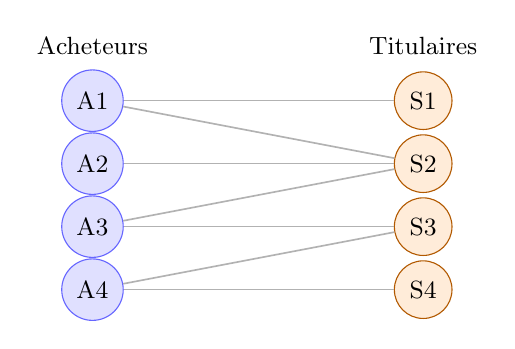
\begin{tikzpicture}[
    buyer/.style={circle, draw=blue!60, fill=blue!12, minimum size=7mm, font=\small},
    supplier/.style={circle, draw=orange!70!black, fill=orange!15, minimum size=7mm, font=\small},
    edge/.style={draw=gray!60, line width=0.6pt}
  ]
    % Titres
    \node[font=\small] at (0, 0.9) {Acheteurs};
    \node[font=\small] at (4.2, 0.9) {Titulaires};

    % Acheteurs (gauche)
    \node[buyer] (a1) at (0, 0.2) {A1};
    \node[buyer] (a2) at (0, -0.6) {A2};
    \node[buyer] (a3) at (0, -1.4) {A3};
    \node[buyer] (a4) at (0, -2.2) {A4};

    % Titulaires (droite)
    \node[supplier] (s1) at (4.2, 0.2) {S1};
    \node[supplier] (s2) at (4.2, -0.6) {S2};
    \node[supplier] (s3) at (4.2, -1.4) {S3};
    \node[supplier] (s4) at (4.2, -2.2) {S4};

    % Arêtes = marchés
    \draw[edge] (a1) -- (s1);
    \draw[edge] (a1) -- (s2);
    \draw[edge] (a2) -- (s2);
    \draw[edge] (a3) -- (s2);
    \draw[edge] (a3) -- (s3);
    \draw[edge] (a4) -- (s3);
    \draw[edge] (a4) -- (s4);
  \end{tikzpicture}
  \caption{Schéma du graphe biparti acheteur–titulaire (arêtes = marchés).}
  \label{fig:bipartite_schema}
\end{figure}

La Figure~\ref{fig:degree} montre la distribution des degrés côté acheteurs et titulaires.
\begin{figure}[t]
  \centering
  \includegraphics[width=0.85\linewidth]{step2_degree_distributions.png}
  \caption{Distributions des degrés (acheteurs vs titulaires).}
  \label{fig:degree}
\end{figure}


\subsection{Features de risque}
Pour chaque relation acheteur–titulaire, nous calculons : (i) degrés acheteur et titulaire, (ii) nombre de marchés entre les deux acteurs, (iii) part du montant de l’arête dans le total acheteur et dans le total titulaire (concentration), (iv) indicateur de concurrence $1/(1+\text{offresRecues})$, (v) intensité financière $\log(1+\text{montant})$.

La Figure~\ref{fig:shares} illustre les distributions de concentration acheteur et titulaire.
\begin{figure}[t]
  \centering
  \includegraphics[width=0.85\linewidth]{step3_edge_share.png}
  \caption{Distributions des parts de concentration (acheteur vs titulaire).}
  \label{fig:shares}
\end{figure}


\subsection{Projection et centralité (PageRank)}
Pour mobiliser un concept vu en cours (centralité), nous projetons le graphe biparti sur les titulaires : deux fournisseurs sont reliés s’ils partagent au moins un acheteur, avec un poids égal au nombre d’acheteurs communs. Nous calculons ensuite le PageRank sur ce graphe projeté afin d’identifier des fournisseurs centraux dans le réseau d’interactions indirectes.

\subsection{Score de risque (baseline)}
Chaque composante est normalisée (min-max), puis combinée avec des poids explicites :
\[
R = 0{,}30 \cdot C_{acheteur} + 0{,}20 \cdot C_{titulaire} + 0{,}20 \cdot N_{marchés} + 0{,}20 \cdot S_{offres} + 0{,}10 \cdot M_{montant}
\]
Les poids sont choisis pour privilégier les signaux de concentration et de faible concurrence, qui sont les plus souvent associés aux risques d’entente. Les autres composantes jouent un rôle de stabilisation afin de ne pas sur-pondérer un seul indicateur.
Le score est un indicateur de tri, pas une preuve de fraude.

\subsection{Reproductibilité}
Les scripts de collecte, de construction du graphe, de calcul des features et de génération des figures sont fournis dans le dépôt (`scripts/`). Les sorties principales sont stockées dans `data/interim/` et `data/processed/`.

\section{Évaluation}
Faute de labels de fraude, l’évaluation est descriptive : (i) distribution du score de risque et quantiles, (ii) comparaison des arêtes “haut risque” vs “faible risque”, (iii) liste des cas prioritaires à inspecter (top-k). Nous vérifions que les “haut risque” cumulent effectivement concentration et faible concurrence, comme attendu par les red flags \citep{OECD2025BidRigging}.

\subsection{Comparaison avec des scores simples}
Nous comparons le score de base à trois scores simplifiés : (i) concentration seule, (ii) concurrence seule, (iii) nombre de marchés seul. Le Tableau~\ref{tab:baseline_compare} rapporte la corrélation de Spearman avec le score de base et l’overlap Jaccard du top 5\% des arêtes (275 relations). Le score de base est le plus proche de la concentration, tout en restant distinct des autres signaux.

\begin{table}[t]
  \centering
  \begin{tabular}{lcc}
    \toprule
    Score alternatif & Spearman vs. baseline & Jaccard top 5\% \\
    \midrule
    Concentration seule & 0.799 & 0.432 \\
    Concurrence seule & 0.487 & 0.093 \\
    Nombre de marchés seul & 0.223 & 0.040 \\
    \bottomrule
  \end{tabular}
  \caption{Comparaison du score de base avec des scores simples.}
  \label{tab:baseline_compare}
\end{table}

\subsection{Analyse de sensibilité des poids}
Nous testons trois configurations de poids : (i) poids équilibrés (0.2 chacun), (ii) concentration renforcée, (iii) concurrence renforcée. Le Tableau~\ref{tab:weight_sensitivity} montre que le classement reste stable (overlap top-20 de 70\% à 90\%), ce qui suggère une robustesse raisonnable aux variations de poids.

\begin{table}[t]
  \centering
  \begin{tabular}{lcc}
    \toprule
    Configuration des poids & Spearman vs. baseline & Overlap top-20 \\
    \midrule
    Équilibrés (0.2 chacun) & 0.975 & 0.70 \\
    Concentration renforcée & 0.987 & 0.90 \\
    Concurrence renforcée & 0.944 & 0.90 \\
    \bottomrule
  \end{tabular}
  \caption{Analyse de sensibilité des poids du score.}
  \label{tab:weight_sensitivity}
\end{table}

La Figure~\ref{fig:riskvsoffers} visualise la relation négative entre score de risque et nombre d’offres reçues.
\begin{figure}[t]
  \centering
  \includegraphics[width=0.85\linewidth]{step7_risk_vs_offers.png}
  \caption{Score de risque vs offres reçues (relation négative attendue).}
  \label{fig:riskvsoffers}
\end{figure}


\FloatBarrier
\section{Résultats}
Nous obtenons 5\,491 arêtes acheteur–titulaire agrégées. La distribution du score est à queue (p95 $\approx$ 0,639 ; p99 $\approx$ 0,732). Les relations “haut risque” ont en moyenne moins d’offres (1,58 vs 3,44) et une concentration très forte ($\approx$ 0,95 côté acheteur). Les corrélations montrent que le score augmente avec la concentration et diminue avec le nombre d’offres. Ces résultats sont cohérents avec l’intuition de collusion, tout en restant non conclusifs.

Le Tableau~\ref{tab:summary} récapitule la taille de l’échantillon et les principaux quantiles du score.
\begin{table}[H]
  \centering
  \begin{tabular}{l r}
    \toprule
    Indicateur & Valeur \\
    \midrule
    Marchés (H2 2024, CPV 4521) & 8\,957 \\
    Acheteurs & 1\,342 \\
    Titulaires & 4\,489 \\
    Arêtes acheteur–titulaire & 5\,491 \\
    Score p95 & 0{,}639 \\
    Score p99 & 0{,}732 \\
    \bottomrule
  \end{tabular}
  \caption{Résumé de l’échantillon et quantiles du score.}
  \label{tab:summary}
\end{table}

\begin{figure}[t]
  \centering
  \includegraphics[width=0.85\linewidth]{step4_risk_score_dist.png}
  \caption{Distribution du score de risque (H2 2024, CPV 4521).}
  \label{fig:riskdist}
\end{figure}

\begin{figure}[t]
  \centering
  \includegraphics[width=0.85\linewidth]{step5_offers_low_vs_high.png}
  \caption{Offres reçues : comparaison entre arêtes à risque faible et élevé (seuil p95).}
  \label{fig:offers}
\end{figure}


La Figure~\ref{fig:top20} présente un exemple de classement (top 20) des relations à risque.
\begin{figure}[t]
  \centering
  \includegraphics[width=0.85\linewidth]{step6_top20_risk.png}
  \caption{Top 20 des scores de risque (anonymisé).}
  \label{fig:top20}
\end{figure}

En complément, la Figure~\ref{fig:pagerank} présente les 10 fournisseurs les plus centraux selon le PageRank sur la projection fournisseurs. Cette mesure ne remplace pas le score de risque, mais apporte un indicateur structurel issu du cours.
\begin{figure}[t]
  \centering
  \includegraphics[width=0.85\linewidth]{step8_pagerank_suppliers.png}
  \caption{Top 10 fournisseurs par PageRank (projection fournisseurs).}
  \label{fig:pagerank}
\end{figure}

\section{Discussion}
Une forte concentration acheteur–titulaire n’est pas nécessairement suspecte : elle peut refléter une spécialisation technique, une proximité géographique ou la structure de marchés locaux à faible nombre d’acteurs. De même, des marchés de faible montant ou très spécifiques peuvent attirer peu d’offres sans qu’il y ait collusion. À l’inverse, la répétition d’attributions entre les mêmes acteurs sur des montants élevés et avec faible concurrence justifie une inspection plus approfondie. Notre score doit donc être interprété comme un outil de priorisation, à compléter par une analyse qualitative et contextuelle.

\section{Limites}
(1) Absence de labels de fraude, (2) données publiques imparfaites, (3) champ limité à CPV 4521 et H2-2024, (4) agrégation qui masque des variations internes, (5) concentration parfois légitime (spécialisation, géographie).

\section{Conclusions et perspectives}
Ce projet montre qu’une modélisation par graphes permet de produire un score de risque simple et interprétable pour la priorisation des contrôles dans les marchés publics. Les résultats indiquent une petite queue d’arêtes fortement concentrées et faiblement concurrentielles, qui mérite une inspection qualitative. Pour aller plus loin, il serait nécessaire d’intégrer les soumissionnaires perdants, les prix des offres, ou des liens juridiques entre entreprises.

\bibliography{references}
\bibliographystyle{iclr2021_conference}

\end{document}
